% Standalone XeLaTeX source. Uses standard commands and distributed packages.
% Source problem: public/notes/物工/問題/2015ap_exam.pdf, PDF pages 4–5.
\documentclass[11pt,a4paper]{article}
\usepackage[margin=24mm]{geometry}
\usepackage{fontspec}
\usepackage{xeCJK}
\setCJKmainfont{HaranoAjiMincho-Regular.otf}
\setCJKsansfont{HaranoAjiGothic-Medium.otf}
\usepackage{amsmath,amssymb}
\usepackage{tikz}
\usetikzlibrary{arrows.meta}
\setlength{\parindent}{1em}
\setlength{\parskip}{0.35em}
\renewcommand{\figurename}{図}
\title{物理工学専攻 院試解答集 ver2\\2015年 物理学I 第2問}
\author{政岡凜太郎}
\date{}
\begin{document}
\maketitle

\section*{[1] リングを貫く磁束}
リングの中心を$(X,0,0)$、面内の中心からの座標を$(u,v)$とする。円盤上では$x=X+u$、$z=0$であり、面積要素の法線を$+z$向きにとると、
\begin{align}
  \Phi(X)&=\int_{u^2+v^2\le a^2} B_0[1+\alpha(X+u)]\,\mathrm d u\,\mathrm d v\\
  &=B_0(1+\alpha X)\pi a^2
    +B_0\alpha\int_{u^2+v^2\le a^2}u\,\mathrm d u\,\mathrm d v\\
  &=\boxed{\pi a^2B_0(1+\alpha X)}.
\end{align}
円盤は$u\mapsto-u$で対称なので、積分中の奇関数$u$の項はゼロである。

\section*{[2] 一定速度で運動するときの電流}
正の面法線を$+z$にとると、正の周回方向は反時計回りである。$X$が速度$V>0$で増えるため、$+z$向きの磁束が増加する。ファラデーの法則
\begin{equation}
  IR=-\frac{\mathrm d\Phi}{\mathrm dt}
\end{equation}
の負号は誘導電流が磁束の増加を妨げることを表す。よって符号付き電流は
\begin{equation}
  \boxed{I=-\frac{\pi a^2B_0\alpha V}{R}}.
\end{equation}
負号は、実際の電流が図の正方向と逆の時計回りであることを示す。

\section*{[3] 一定速度を保つための力}
電流が流れるリングに働く磁気力は、周回方向の電流要素と磁場とのローレンツ力から求まる。円周上の角度を$\vartheta$とすると、正の周回方向の電流要素は$\mathrm d\boldsymbol\ell=a(-\sin\vartheta,\cos\vartheta,0)\,\mathrm d\vartheta$である。リング上では$z=0$、$x=X+a\cos\vartheta$なので、$\mathrm d\boldsymbol F=I\,\mathrm d\boldsymbol\ell\times\boldsymbol B$より
\begin{align}
  \mathrm dF_{\mathrm{mag},x}
  &=IaB_0\cos\vartheta[1+\alpha(X+a\cos\vartheta)]\,\mathrm d\vartheta,\\
  F_{\mathrm{mag},x}
  &=IaB_0\int_0^{2\pi}
    [(1+\alpha X)\cos\vartheta+\alpha a\cos^2\vartheta]\,\mathrm d\vartheta
    =I\pi a^2B_0\alpha.
\end{align}
ここで$B_z$の一様部分の寄与は一周積分で相殺し、$x$に比例する部分だけが残る。したがって一定速度では、加えた外力がこの磁気抵抗力とつり合う。外力の大きさは
\begin{equation}
  \boxed{F=\frac{(\pi a^2B_0\alpha)^2}{R}V}.
\end{equation}
この結果は電力でも確認できる。外力の仕事率$FV$は$RI^2$に等しい。

\section*{[4] 時間変化する磁場と運動方程式}
磁束は
\begin{equation}
  \Phi(X,t)=\pi a^2B_0b(t)(1+\alpha X)
\end{equation}
である。正の電流を反時計回りとする規約を保つと、起電力と電流は
\begin{equation}
  IR=-\frac{\mathrm d\Phi}{\mathrm dt}
  =-\pi a^2B_0\frac{\mathrm d}{\mathrm dt}[b(t)(1+\alpha X)].
  \label{eq:current}
\end{equation}
角度$\vartheta$の電流要素を
$\mathrm d\boldsymbol\ell=a(-\sin\vartheta,\cos\vartheta,0)\,\mathrm d\vartheta$
とすると、$\mathrm d\boldsymbol F=I\,\mathrm d\boldsymbol\ell\times\boldsymbol B$である。$x=X+a\cos\vartheta$を代入して一周積分すると、$x$成分は
\begin{equation}
  F_{\mathrm{mag},x}=I\pi a^2B_0\alpha b(t),
\end{equation}
となる。運動方程式$m\ddot X=F_{\mathrm{mag},x}$に式\eqref{eq:current}を代入すると
\begin{equation}
  m\ddot X=-\frac{(\pi a^2B_0)^2\alpha}{R}
  b(t)\frac{\mathrm d}{\mathrm dt}[b(t)(1+\alpha X)].
\end{equation}
したがって問題文の形では
\begin{equation}
  \boxed{\alpha\ddot X=-\lambda b(t)\frac{\mathrm d}{\mathrm dt}[b(t)(1+\alpha X)]},
  \qquad
  \boxed{\lambda=\frac{(\pi a^2B_0\alpha)^2}{mR}}.
\end{equation}
$\lambda$の次元は時間の逆数である。

\section*{[5] べき級数の初期係数}
$0\le t<\tau$では$b(t)=t/\tau$だから、運動方程式は
\begin{equation}
  \alpha\ddot X=-\frac{\lambda t}{\tau^2}
  \left(1+\alpha X+\alpha t\dot X\right).
  \label{eq:series-eq}
\end{equation}
初期条件$X(0)=0$、$\dot X(0)=0$を
$X=\sum_{k=0}^{\infty}a_kt^k$に適用すると、$a_0=a_1=0$である。式\eqref{eq:series-eq}の$t^0$の係数を比べると、左辺は$2\alpha a_2$、右辺はゼロなので、$a_2=0$となる。

\section*{[6] 短時間近似での速度}
式\eqref{eq:series-eq}の$t^1$の係数を比べ、$a_0=0$を使うと
\begin{equation}
  6\alpha a_3=-\frac{\lambda}{\tau^2},
  \qquad
  \boxed{a_3=-\frac{\lambda}{6\alpha\tau^2}}.
\end{equation}
問題文の$\tau\ll1/\lambda$の近似では$X\simeq a_3t^3$なので、$t=\tau$での速度は
\begin{equation}
  \boxed{V_0=\dot X(\tau)\simeq3a_3\tau^2=-\frac{\lambda}{2\alpha}}.
\end{equation}
負号はリングが初期位置から$-x$方向へ動くことを表す。

\section*{[7] 最終位置}
$t\ge\tau$では$b(t)=1$であり、運動方程式は
\begin{equation}
  \ddot X+\lambda\dot X=0.
\end{equation}
したがって速度は$\dot X(t)=V_0e^{-\lambda(t-\tau)}$と減衰し、無限時間後の変位は$V_0/\lambda$である。設問[6]--[7]で指定された三次近似$X\simeq a_3t^3$を用いると、
\begin{equation}
  X(\tau)\simeq-\frac{\lambda\tau}{6\alpha},\qquad
  V_0\simeq-\frac{\lambda}{2\alpha}.
\end{equation}
従って、この指定された近似の下での答えは
\begin{equation}
  \boxed{X(\infty)\simeq X(\tau)+\frac{V_0}{\lambda}
    =-\frac{1}{2\alpha}-\frac{\lambda\tau}{6\alpha}}.
\end{equation}

この三次近似の結果と、運動方程式の漸近展開の精度は区別する必要がある。$\epsilon=\lambda\tau$、$u=t/\tau$、$y=\alpha X$と置くと、$0\le u\le1$で式\eqref{eq:series-eq}は
\begin{equation}
 y''(u)=-\epsilon u[1+y(u)+uy'(u)],\qquad y(0)=y'(0)=0
\end{equation}
となる。この有限区間の線形初期値問題を$\epsilon$で順に展開すると
\begin{equation}
 y(u)=-\frac{\epsilon u^3}{6}+\frac{\epsilon^2u^6}{45}+O(\epsilon^3),\qquad
 y'(u)=-\frac{\epsilon u^2}{2}+\frac{2\epsilon^2u^5}{15}+O(\epsilon^3)
\end{equation}
を得る。従って$X(\tau)=y(1)/\alpha$、$V_0/\lambda=y'(1)/(\alpha\epsilon)$を足した漸近展開は
\begin{equation}
 X(\infty)=-\frac{1}{2\alpha}-\frac{\lambda\tau}{30\alpha}
 +O\!\left(\frac{(\lambda\tau)^2}{\alpha}\right).
\end{equation}
三次近似だけで得た箱内の一次係数$-1/6$は、$V_0$の次の補正を含めないため、この漸近展開の一次係数とは異なる。

\begin{figure}[htbp]
\centering
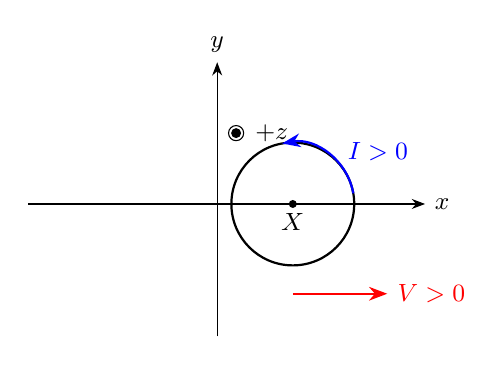
\begin{tikzpicture}[>=Stealth,scale=1.2,font=\small]
  % Schematic display scale; the circle and current direction are derived together.
  \pgfmathsetmacro{\ringX}{0.8}
  \pgfmathsetmacro{\ringR}{0.65}
  \pgfmathsetmacro{\arcStart}{10}
  \pgfmathsetmacro{\arcEnd}{100}
  \draw[->] (-2,0)--(2.2,0) node[right] {$x$};
  \draw[->] (0,-1.4)--(0,1.5) node[above] {$y$};
  \draw[thick] (\ringX,0) circle (\ringR);
  \fill (\ringX,0) circle (1.2pt);
  \node[below] at (\ringX,0) {$X$};
  \draw[->,blue,thick] (\ringX,0) ++({\ringR*cos(\arcStart)},{\ringR*sin(\arcStart)})
    arc[start angle=\arcStart,end angle=\arcEnd,radius=\ringR];
  \node[blue] at (1.7,0.55) {$I>0$};
  \draw (0.2,0.75) circle (0.08);
  \fill (0.2,0.75) circle (1.5pt);
  \node[right] at (0.3,0.75) {$+z$};
  \draw[->,red,thick] (\ringX,-0.95)--({\ringX+1},-0.95) node[right] {$V>0$};
\end{tikzpicture}
\caption{磁束と電流の符号規約。紙面の手前が$+z$、正電流はその向きから見て反時計回り。}
\label{fig:ring}
\end{figure}

\end{document}
